\section{Assessing the Performance Impact}

\label{sec:predictimprove}
%\todo{Adding a picture, maybe similar to Sammati paper}
%\todo{memory bound. Predict memory bound. IO we can't bound. original 100, we remove 80. Latency can be predict to the execution time.  } 
Fixing false sharing does not necessarily yield significant performance speedup, even for instances with a large number of cache invalidations~\cite{Sheriff, Predator}. Zhao et. al. observe that fixing false sharing may even slowdown a program because of excessive memory consumption or the lose of locality~\cite{qinzhao}. Reporting insignificant false sharing instances are not false positives, but that can increase manual burden for programmers.

To solve this problem, \cheetah{} makes the first attempt to quantitatively assess the potential performance gain of fixing a false sharing instance. Thus, programmers can focus on severe problems only, avoiding unnecessary manual effort.

\cheetah{}'s assessment is based on the following observations:

\begin{itemize}
\item {\bf Observation 1:} the sampling is evenly distributed over the whole execution. Based on this, we can use the sampling to represent the whole execution. The similar idea is widely used by exiting work like Oprofile and Gprof, when they identify the hotspots of function calls and code~\cite{oprofile, DBLP:conf/sigplan/GrahamKM82}.

\item {\bf Observation 2:} The PMU provides the latency information (e.g. cycles) of each memory operation. We also observe that the latency of accessing falsely shared objects is significantly higher than that of normal accesses. 

\end{itemize}

Based on these two observations, {\bf we propose to use the sampled cycles to represent the runtime of an execution and further predict the performance impact of a falsely-shared object}. The assessment is performed in three steps listed as follows. 

\begin{itemize}
\item \cheetah{} first predicts the possible cycles of a falsely-shared object after fixes, as discussed in Section~\ref{sec:impactobject}. 

\item Then \cheetah{} assesses the performance impact on the related threads brought by fixes, which is discussed in Section~\ref{sec:impactthread}. 
 
\item In the end, \cheetah{} assesses the performance impact on the application in Section~\ref{sec:impactapp}. 
\end{itemize}

The remainder of this section discusses the detailed assessment step by step. For the simplicity reason, we abbreviate the falsely-shared object as ``$O$'', the related thread as ``$t$'', the prediction as ``$Pred$'', the runtime as ``$RT$'', the application as ``$App$''. 

\subsection{Impact on Accesses of the Object}
\label{sec:impactobject}

In the first step, \cheetah{} predicts the possible cycles of accesses after fixing false sharing of the object $O$.  \cheetah{} collects total cycles of accesses --- $Cycles\_O$ and total number of accesses --- $Accesses\_O$. 

Since it is impossible to know the average cycles of every access after fixing --- $AverCycles\_{nofs}$ --- without actual fixes, {\it \cheetah{} utilizes the average cycles of the serial phases ($AverCycles\_{serial}$) to approximate this value}. Because there is no false sharing in serial phases, $AverCycles\_{serial}$ represents the least number of cycles for memory accesses after fixing any false sharing instance. In reality, $AverCycles\_{nofs}$ maybe is larger than $AverCycles\_{serial}$ since fixing false sharing may lead to excessive memory consumption or the lose of locality~\cite{qinzhao}. \cheetah{} actually predicts the best performance of fixing every false sharing instance. 
 
 \cheetah{} computes the total cycles of accesses after fixing ($PredCycles\_{O}$) according to EQ.(\ref{eq:predictedcyclesofo}).  It is expected that $PredCycles\_{O}$ will be less than the total cycles before fixing --- $Cycles_O$, since fixing a false sharing problem can reduce the execution time.  

\begin{equation}
\label{eq:predictedcyclesofo}
 PredCycles\_{O} = (AverCycles\_{nofs} * Accesses\_O)
\end{equation} 

\subsection{Impact on Related Threads}
\label{sec:impactthread}

The second step is to assess how reducing the access cycles of $O$ (with $PredCycles\_{O}$) can potentially affect the execution time of its related threads. 

\Cheetah{} collects the following information of every thread: the execution time --- $RT\_{t}$, the total number of accesses --- $Accesses\_{t}$, and the total cycles of all memory accesses --- $Cycles\_{t}$. \cheetah{} lets every thread to respond the signal handler of its sampling, and records the number of accesses and cycles correspondingly. To collect $RT\_{t}$, \cheetah{} intercepts the creation of threads by passing a custom function as the start routine. In this custom function, \cheetah{} uses the RDTSC (ReaD-Time Stamp Counter) to track the execution time of every thread --- $RT\_{t}$. 
%To gather the number of accesses and cycles of every thread, \cheetah{} makes every thread to respond the signal handler and records the number of accesses and cycles correspondingly. 

After the collection, \cheetah{} predicts the cycles of every related thread --- $PredCycles\_{t}$ --- after fixes as the EQ.(\ref{eq:predictedcyclesofthread}). 

\begin{equation}
\label{eq:predictedcyclesofthread}
 PredCycles\_{t} = Cycles\_{t} - Cycles\_{O} + PredCycles\_{O} 
\end{equation} 
 
Based on $PredCycles\_{t}$, \cheetah{} assesses the predicted runtime of a thread --- $PredRT_{t}$ --- as the EQ.(\ref{eq:predictedrtofthread}). We assume that {\bf the execution time is proportional to the cycles of accesses} so that the less of cycles indicates the less of the execution time and a performance speedup. It is expected that fixing the false sharing problem inside the object $O$ will improve the performance for its related threads. 

\begin{equation}
\label{eq:predictedrtofthread}
 PredRT\_{t} = (PredCycles\_{t} / Cycles\_{t}) * RT\_{t} 
\end{equation} 

\subsection{Impact on the Application}
\label{sec:impactapp}

In the end, \cheetah{} assesses how fixing will change the performance of the application. 

Actually, improving the performance of one thread may not increase the final performance if this thread is not in the critical path.  To simplify the prediction and verify our idea, \cheetah{} currently focuses on applications with the normal fork-join model shown as Figure~\ref{fig:forkjoinmodel}. This model is the most important and widely used model in reality. All applications that we have evaluated in this paper utilize this fork-join model. The performance assessment will be more complicated if nested threads exist inside an application. 


\begin{figure*}[ht!]
\begin{center}
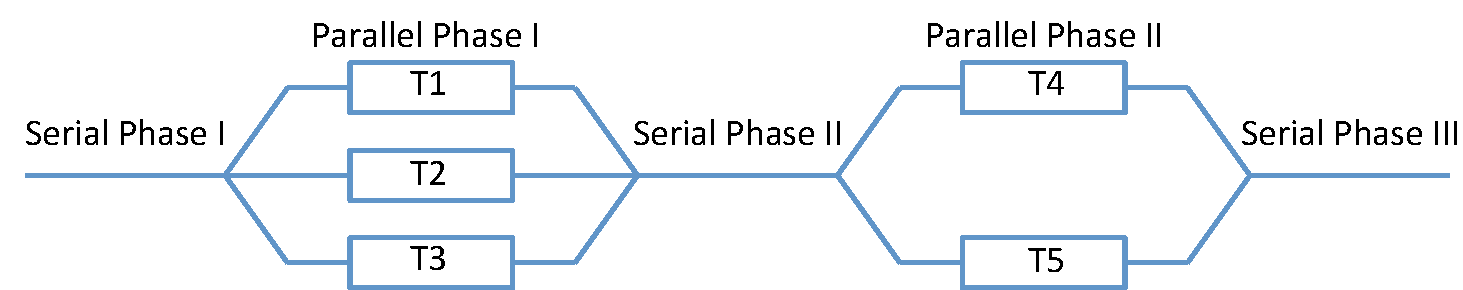
\includegraphics[width=6in]{figure/forkjoin}
\end{center}
\caption{The fork-join model that \Cheetah{} currently focuses on to assess the performance impact of false sharing instances. }
\label{fig:forkjoinmodel}
\end{figure*}

\cheetah{} tracks the creations and joins of threads in order to verify whether an application belongs to the fork-join model or not. \Cheetah{} also collects the execution time of different serial and parallel phases, using RDTSC (ReaD-Time Stamp Counter) available on X86 machines~\cite{rtdsc}. As shown in Figure~\ref{fig:forkjoinmodel}, an application leaves a serial phase after a thread creation and it leaves a parallel phase after all children threads created in this parallel pahse are joined successfully. 

Based on the runtime information about every parallel phase and serial phase, \cheetah{} can assess the final performance impact by recomputing the length of each phase and the total time after fixing: the length of each phase is decided by the thread with the longest execution time, while the total time of an application is equal to the sum of different parallel phases and serial phases. 

After \cheetah{} computes the possible execution time of an application after fixing a false sharing problem, \cheetah{} will compute the potential performance improvement based on EQ.(\ref{eq:improvement}). We will report the potential performance improvement for every falsely-shared object as Figure~\ref{fig:lr}. Then programmers can focus only on those ones with serious performance impact. We further verify the precision of \cheetah{}'s assessment in Section~\ref{sec:precision}.

\begin{equation}
\label{eq:improvement}
PerfImprove = RT\_{App} / PredRT\_{App}
\end{equation}

%We will uses an example to show that. For example, there is a false sharing problem that will involved in the $T1$ and $T2$ of Figure~\ref{fig:forkjoinmodel}, but not other threads.  We will assess the possible runtime of $PredictRT_{T1}$ and $PredictRT_{T2}$. Then we checked that whether these predicted runtime will affect the runtime of parallel phase I by checking whether these two runtime are less than the runtime of $T3$ at first. If it won't, then fixing the false sharing problem won't affect the final performance. Otherwise, we have to recompute the length of parallel phase I, while the length of other phases will keep the same. By doing that, we will get a new runtime for the application. Using the EQ.(\ref{eq:improvement}), we can compute the potential performance improvement of this application by fixing the false sharing problems related to the thread $T1$ and $T2$. 









